\section{Pipeline}
\label{sec:pipeline}

Eine schematische \"Ubersicht der in diesem Projekt eingesetzten
zweistufigen Vorhersagepipeline ist in Abbildung~\ref{fig:pipeline}
dargestellt.

Die Pipeline ist so aufgebaut, dass auf eine Bildeingabe zun\"achst
eine Bildsegmentierung angewendet wird, um den Bereich des Bildes,
welcher das Nummernschild enth\"alt, herauszutrennen.
F\"ur die Bildsegmentierung wurde ein neuronales Netz trainiert,
die Einzelheiten des Verfahrens werden in Abschnitt~\ref{sec:bildsegmentierung}
n\"aher beschrieben.

Nach der Bildsegmentierung wird auf den herausgetrennten Bereich eine
Texterkennung angewendet, um die Zeichenfolge des Nummernschildes
zu extrahieren. Dieses Verfahren wird in Abschnitt~\ref{sec:texterkennung}
beschrieben.

\begin{figure}[h]
    \centering
    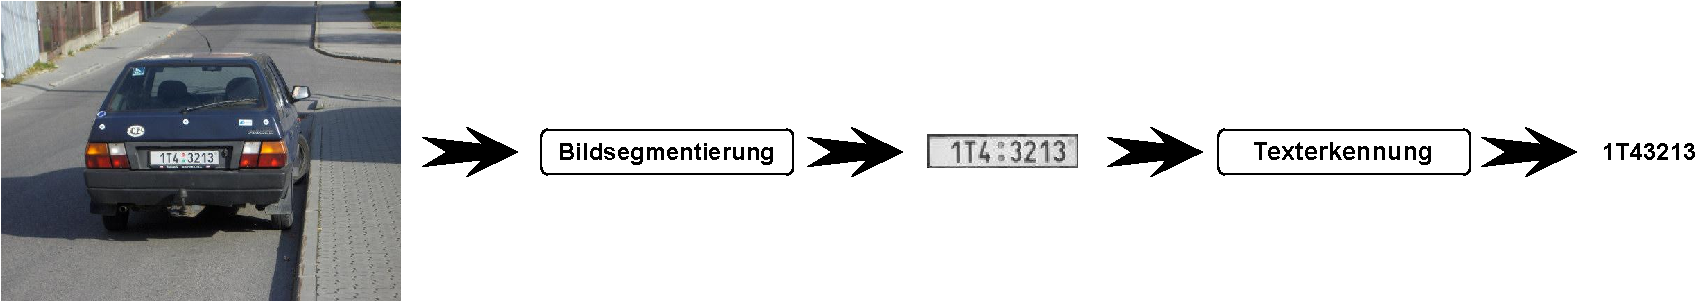
\includegraphics[width=\textwidth]{abbildungen/pipeline}
    \caption{Schematische Darstellung der zweistufigen Vorhersagepipeline.
        Zun\"achst wird das Nummernschild mithilfe von Bildsegmentierung
        extrahiert. Anschlie{\ss}end werden die Zeichen durch Texterkennung
        ausgelesen.}
    \label{fig:pipeline}
\end{figure}

\subsection{Bildsegmentierung}
\label{sec:bildsegmentierung}

Das Ziel einer Bildsegmentierung ist es, die relevanten Bereiche eines
Bildes von den restlichen zu trennen.
In dieser Situation ist es also gefordert, den Bereich des Bildes,
welcher das Nummernschild enth\"alt, vom Rest des Bildes zu trennen.

Zu diesem Zweck kommt in diesem Projekt eine bin\"are Klassifikation
zum Einsatz: F\"ur jeden Pixel des Eingabebildes wird klassifiziert,
ob er Teil des Nummernschildes ist, oder nicht.
Das Ziel ist es also, f\"ur ein Eingabebild eine bin\"are Maske vorherzusagen,
welche f\"ur jeden Pixel eine 1 enth\"alt, falls er Teil des Nummernschildes
ist und anderenfalls eine 0.
Eine visuelle Darstellung dieses Konzeptes ist in
Abbildung~\ref{fig:binaere-maske} gegeben.

\begin{figure}[h]
    \centering
    \begin{subfigure}{0.495\textwidth}
        \centering
        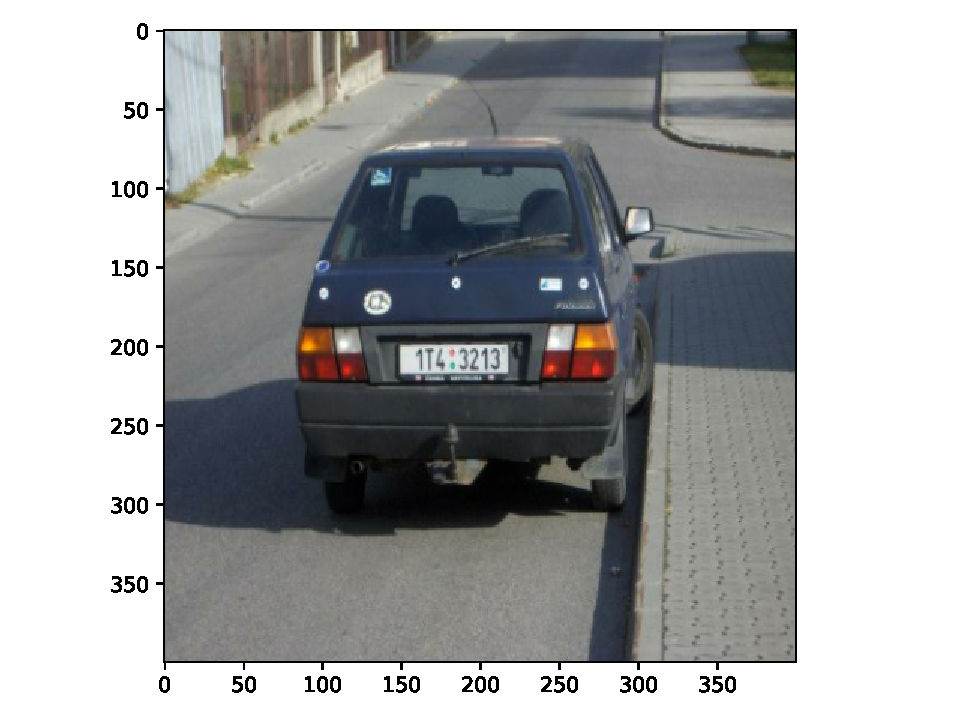
\includegraphics[width=\textwidth]{abbildungen/segmentation_input}
        \caption{Eingabebild}
    \end{subfigure}
    \begin{subfigure}{0.495\textwidth}
        \centering
        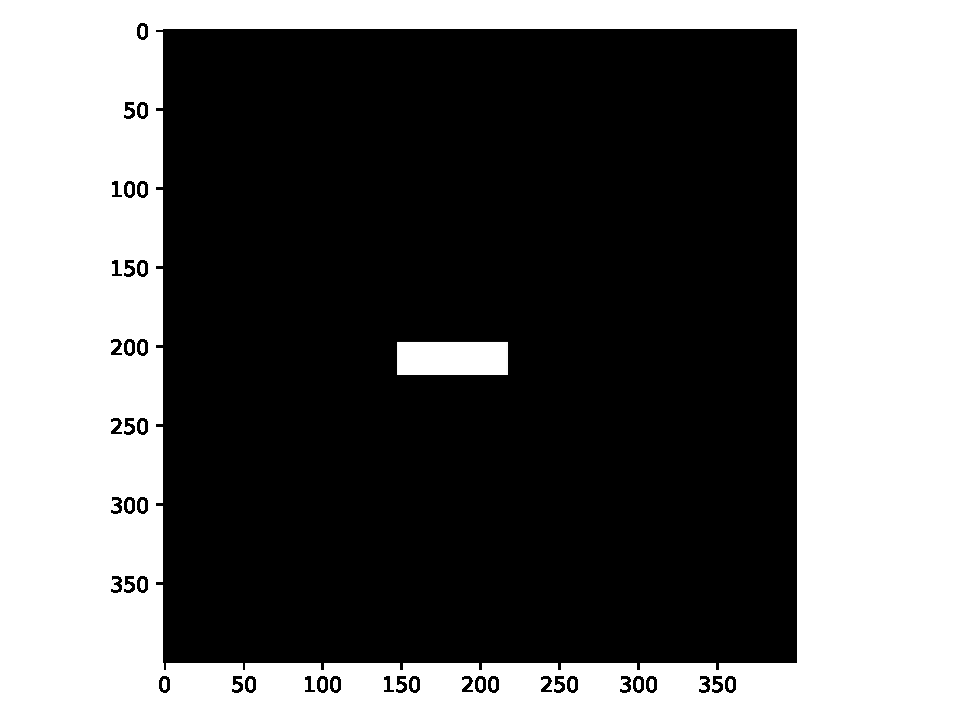
\includegraphics[width=\textwidth]{abbildungen/segmentation_output}
        \caption{Bin\"are Maske des Nummernschildes.}
    \end{subfigure}
    \caption{Die bin\"are Maske (rechts) ordnet jedem Pixel der Eingabe
        (links) einen Wert 1 (hier wei{\ss} dargestellt) zu, falls sich dieser
        im Nummernschild befindet. Andernfalls wird ein Wert von 0 (schwarz)
        zugeordnet.}
    \label{fig:binaere-maske}
\end{figure}

Als Klassifikationsverfahren kommen zu diesem Zweck CNNs zum Einsatz,
die bereits in Abschnitt~\ref{sec:cnns} beschrieben wurden.
Auf die genaue Architektur und die Funktionsweise von CNNs bez\"uglich
Klassifikation soll nun genauer eingegangen werden.

\subsubsection{Nummernschildextraktion mit CNNs}

Wie schon in Abschnitt~\ref{sec:neuronale-netze} erl\"autert, ordnen
neuronale Netze einer Eingabe fester Gr\"o{\ss}e eine zugeh\"orige
Ausgabe fester Gr\"o{\ss}e zu.
In diesem Fall soll die Ausgabe des Netzes zu einem Eingabebild
genau die bin\"are Maske sein, welche das Nummernschild repr\"asentiert.
Da die Bilder im Datensatz allerdings verschiedene Aufl\"osungen
und damit auch verschiedene Gr\"o{\ss}en aufweisen, neuronale Netze
aber auf eine feste einheitliche Gr\"o{\ss}e angewiesen sind,
m\"ussen die Bilder vor der Eingabe in das neuronale Netz
zun\"achst auf eine einheitliche Gr\"o{\ss}e gebracht werden.
In diesem Projekt wird zu diesem Zweck jedes Bild vor der Eingabe
in das Netz auf eine Gr\"o{\ss}e von 400x400 skaliert.
Die insgesamt bei diesem Projekt zum Einsatz kommende Architektur des
neuronalen Netzes wird nun kurz beschrieben.

Eine schematische \"Ubersicht der Netzarchitekturist in
Abbildung~\ref{fig:netzarchitektur} gegeben. Die Details zu jeder
Schicht sind in Tabelle~\ref{tab:netzarchitektur} aufgef\"uhrt.

\begin{figure}[h]
    \centering
    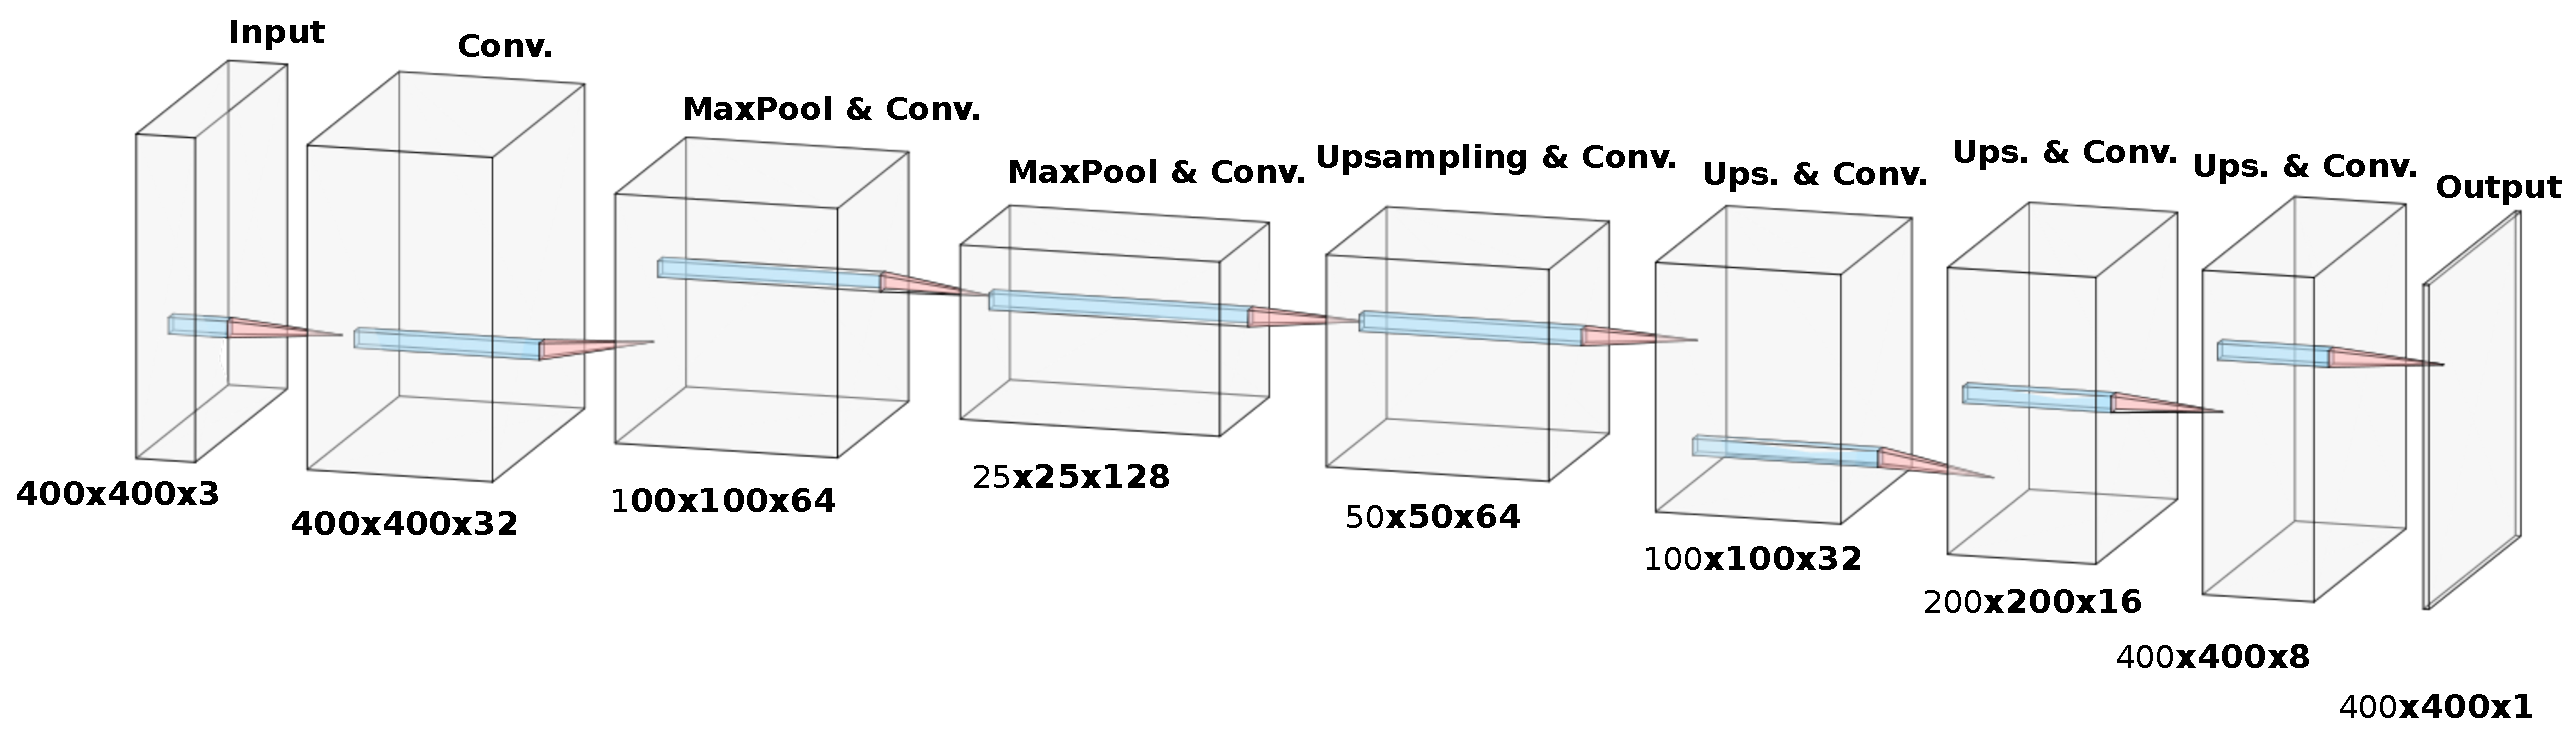
\includegraphics[width=\textwidth]{abbildungen/network_architecture}
    \caption{Schematische Darstellung der gew\"ahlten Netzarchitektur
        zur Bildsegmentierung.}
    \label{fig:netzarchitektur}
\end{figure}

\begin{table}
    \centering
    \caption{Die eingesetzte Netzarchitektur.}
    \label{tab:netzarchitektur}
    \begin{tabular}{|l|l|l|}
        \hline

        \textbf{Schicht}                      & \textbf{Ausgabegr\"o{\ss}e} & \textbf{Anzahl Parameter} \\

        \hline

        Eingabe                               & 400x400x3                   & 0                         \\

        \hline

        Faltungsschicht, 32 3x3 Kernel, ReLU  & 400x400x32                  & 896                       \\

        \hline

        Max-Pooling, 4x4 Kernel               & 100x100x32                  & 0                         \\

        \hline

        Faltungsschicht, 64 3x3 Kernel, ReLU  & 100x100x64                  & 18496                     \\

        \hline

        Max-Pooling, 4x4 Kernel               & 25x25x64                    & 0                         \\

        \hline

        Faltungsschicht, 128 3x3 Kernel, ReLU & 25x25x128                   & 73856                     \\

        \hline

        Upsampling                            & 50x50x128                   & 0                         \\

        \hline

        Faltungsschicht, 64 3x3 Kernel, ReLU  & 50x50x64                    & 73792                     \\

        \hline

        Upsampling                            & 100x100x64                  & 0                         \\

        \hline

        Faltungsschicht, 32 3x3 Kernel, ReLU  & 100x100x32                  & 18464                     \\

        \hline

        Upsampling                            & 200x200x32                  & 0                         \\

        \hline

        Faltungsschicht, 16 3x3 Kernel, ReLU  & 200x200x16                  & 4624                      \\

        \hline

        Upsampling                            & 400x400x16                  & 0                         \\

        \hline

        Faltungsschicht, 8 3x3 Kernel, ReLU   & 400x400x8                   & 1160                      \\

        \hline

        Faltungsschicht, 1 3x3 Kernel, ReLU   & 400x400x1                   & 9                         \\

        \hline
    \end{tabular}
\end{table}

\subsection{Texterkennung}
\label{sec:texterkennung}